\documentclass[12pt, letterpaper]{article}
\usepackage[utf8]{inputenc}
\usepackage[letterpaper, margin=3.cm]{geometry}
\usepackage{graphicx}
\graphicspath{{/home/clebson/Documents/ComplexNetworksDCC/tp3/img//}}

\usepackage{epstopdf}
\epstopdfsetup{outdir=./}


\title{Experiment with NetLogo: Report}
\author{Clebson C. A. de Sá}

\begin{document}
\maketitle

Questão 1: A primeira questão pede para considerar o modelo ``Small-World``.
A análise consistiu em uma rede baseada em 40 nós, no qual uma série de experimentos
foram realizados no software NetLogo com o intuíto de entender as características 
da rede.
A primeira observação a ser feita é que as conexões de cada nó levam em 
consideração a probabilidade de conexão entre os nós. No programa é possível
indicar a probabilidade que deseja avaliar por meio da variação do 
parâmetro ``rewiring-probability''.
As ligações são aleatoriamente proporcionais a esta probabilidade. Assim sendo,
para se ter uma boa estimativa deste parâmetro fiz vários testes considerando 
10 repetições para as probabilidades com um intervalo de 0.1 no intervalo
$\left[0.1, 0.9\right]$ com o intuito de computar o desvio padrão e entender melhor
a variação em relação a média. 
Os resultados para este experimento pode ser visualizado
na Figura \ref{fig:small-world}.

\begin{figure*}[h]
  \centering
  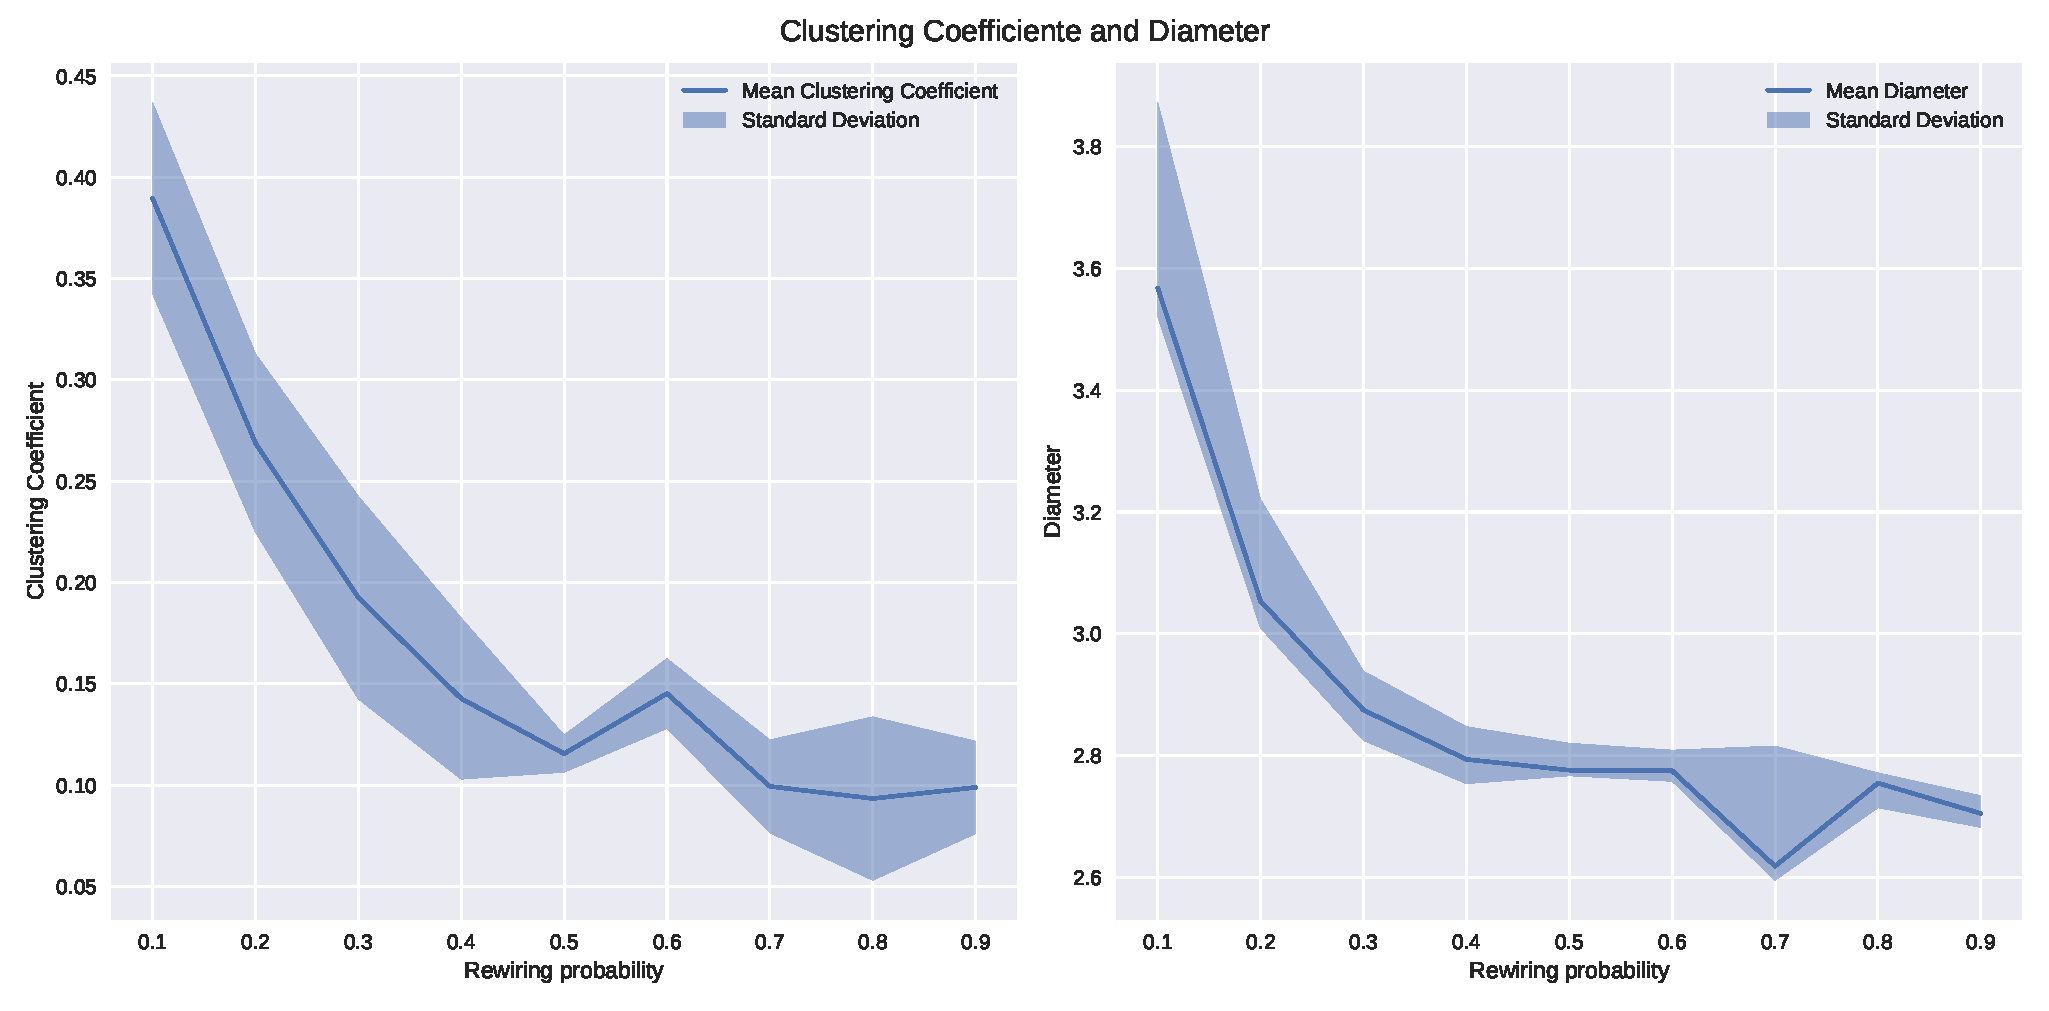
\includegraphics[scale=0.4]{graphProb1.pdf}
  \caption{Coeficiente de Clusterização e Diâmetro com variação da probabilidade.}
  \label{fig:small-world}
\end{figure*}


Conforme podemos visualizar nesta figura, os valores para o Coeficiente de Clusterização
e Diâmetro diminuem conforme aumenta-se a probabilidade de linkagem entre os nós.
Isto é explicato devido ao aumento da quantidade de links  entre os nós.
Observando os gráficos podemos também assumir que conforme a probabilidade se aproxima
do máximo existe uma estabilização das métricas sendo analisadas.


Questão 2:




\end{document}
